% Shrani samo to v graf_matriki.tex
$\vcenter{\hbox{
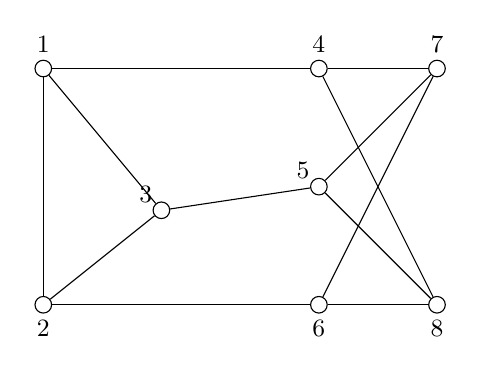
\begin{tikzpicture}[
    vertex/.style={circle, draw=black, fill=white, inner sep=0pt, minimum size=6pt, font=\small},
    lbl/.style={font=\small}
]
    % --- 1. DEL: GRAF ---
    \node[vertex] (v1) at (0,3) {}; \node[lbl] at (0,3.3) {1};
    \node[vertex] (v2) at (0,0) {}; \node[lbl] at (0,-0.3) {2};
    \node[vertex] (v3) at (1.5,1.2) {}; \node[lbl] at (1.3,1.4) {3};

    \node[vertex] (v4) at (3.5,3) {}; \node[lbl] at (3.5,3.3) {4};
    \node[vertex] (v5) at (3.5,1.5) {}; \node[lbl] at (3.3,1.7) {5};
    \node[vertex] (v6) at (3.5,0) {}; \node[lbl] at (3.5,-0.3) {6};

    \node[vertex] (v7) at (5,3) {}; \node[lbl] at (5,3.3) {7};
    \node[vertex] (v8) at (5,0) {}; \node[lbl] at (5,-0.3) {8};

    \draw (v1) -- (v2); \draw (v1) -- (v3); \draw (v2) -- (v3);
    \draw (v1) -- (v4); \draw (v2) -- (v6); \draw (v3) -- (v5);
    \draw (v4) -- (v7); \draw (v4) -- (v8);
    \draw (v5) -- (v7); \draw (v5) -- (v8);
    \draw (v6) -- (v7); \draw (v6) -- (v8);
\end{tikzpicture}
}}
\quad \ \ A = \begin{bmatrix}
\hspace{4pt} 0 & 1 & 1 & 1 & 0 & 0 & 0 & 0 \hspace{4pt} \\
\hspace{4pt} 1 & 0 & 1 & 0 & 0 & 1 & 0 & 0 \hspace{4pt} \\
\hspace{4pt} 1 & 1 & 0 & 0 & 1 & 0 & 0 & 0 \hspace{4pt} \\
\hspace{4pt} 1 & 0 & 0 & 0 & 0 & 0 & 1 & 1 \hspace{4pt} \\
\hspace{4pt} 0 & 0 & 1 & 0 & 0 & 0 & 1 & 1 \hspace{4pt} \\
\hspace{4pt} 0 & 1 & 0 & 0 & 0 & 0 & 1 & 1 \hspace{4pt} \\
\hspace{4pt} 0 & 0 & 0 & 1 & 1 & 1 & 0 & 0 \hspace{4pt} \\
\hspace{4pt} 0 & 0 & 0 & 1 & 1 & 1 & 0 & 0 \hspace{4pt}
\end{bmatrix}
\quad \ \ B = \begin{bmatrix}
\hspace{4pt} \tikznode{b11}{0} & 1 & \tikznode{b13}{1} & 0 & 0 & 0 & 0 & 0 \hspace{4pt} \\
\hspace{4pt} 1 & 0 & 1 & 0 & 0 & 0 & 0 & 0 \hspace{4pt} \\
\hspace{4pt} \tikznode{b31}{1} & 1 & \tikznode{b33}{0} & 0 & 0 & 0 & 0 & 0 \hspace{4pt} \\
\hspace{4pt} 0 & 0 & 0 & \tikznode{b44}{0} & 1 & \tikznode{b46}{1} & 0 & 0 \hspace{4pt} \\
\hspace{4pt} 0 & 0 & 0 & 1 & 0 & 1 & 0 & 0 \hspace{4pt} \\
\hspace{4pt} 0 & 0 & 0 & \tikznode{b64}{1} & 1 & \tikznode{b66}{0} & 0 & 0 \hspace{4pt} \\
\hspace{4pt} 0 & 0 & 0 & 0 & 0 & 0 & \tikznode{b77}{0} & \tikznode{b78}{2} \hspace{4pt} \\
\hspace{4pt} 0 & 0 & 0 & 0 & 0 & 0 & \tikznode{b87}{2} & \tikznode{b88}{0} \hspace{4pt}
\end{bmatrix}
$
\begin{tikzpicture}[remember picture, overlay]
    \draw[black, line width=0.5pt] ([xshift=-2pt, yshift=3pt]b11.north west) rectangle ([xshift=2pt, yshift=-2.5pt]b33.south east);
    \draw[black, line width=0.5pt] ([xshift=-2pt, yshift=3pt]b44.north west) rectangle ([xshift=2pt, yshift=-2.5pt]b66.south east);
    \draw[black, line width=0.5pt] ([xshift=-2pt, yshift=3pt]b77.north west) rectangle ([xshift=2pt, yshift=-2.5pt]b88.south east);
\end{tikzpicture}